% Created by tikzDevice version 0.12.6 on 2026-08-03 03:40:55
% !TEX encoding = UTF-8 Unicode
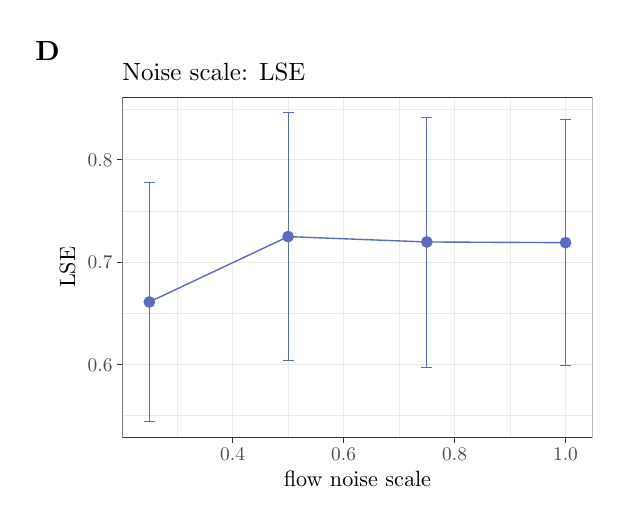
\begin{tikzpicture}[x=1pt,y=1pt]
\definecolor{fillColor}{RGB}{255,255,255}
\path[use as bounding box,fill=fillColor,fill opacity=0.00] (0,0) rectangle (206.87,171.36);
\begin{scope}
\path[clip] (  0.79,  1.87) rectangle (206.08,169.49);
\definecolor{drawColor}{RGB}{255,255,255}
\definecolor{fillColor}{RGB}{255,255,255}

\path[draw=drawColor,line width= 0.4pt,line join=round,line cap=round,fill=fillColor] (  0.79,  1.87) rectangle (206.08,169.49);
\end{scope}
\begin{scope}
\path[clip] ( 34.25, 23.34) rectangle (204.08,146.20);
\definecolor{fillColor}{RGB}{255,255,255}

\path[fill=fillColor] ( 34.25, 23.34) rectangle (204.08,146.20);
\definecolor{drawColor}{gray}{0.92}

\path[draw=drawColor,line width= 0.2pt,line join=round] ( 34.25, 31.23) --
	(204.08, 31.23);

\path[draw=drawColor,line width= 0.2pt,line join=round] ( 34.25, 68.16) --
	(204.08, 68.16);

\path[draw=drawColor,line width= 0.2pt,line join=round] ( 34.25,105.10) --
	(204.08,105.10);

\path[draw=drawColor,line width= 0.2pt,line join=round] ( 34.25,142.04) --
	(204.08,142.04);

\path[draw=drawColor,line width= 0.2pt,line join=round] ( 54.00, 23.34) --
	( 54.00,146.20);

\path[draw=drawColor,line width= 0.2pt,line join=round] ( 94.10, 23.34) --
	( 94.10,146.20);

\path[draw=drawColor,line width= 0.2pt,line join=round] (134.20, 23.34) --
	(134.20,146.20);

\path[draw=drawColor,line width= 0.2pt,line join=round] (174.31, 23.34) --
	(174.31,146.20);

\path[draw=drawColor,line width= 0.4pt,line join=round] ( 34.25, 49.70) --
	(204.08, 49.70);

\path[draw=drawColor,line width= 0.4pt,line join=round] ( 34.25, 86.63) --
	(204.08, 86.63);

\path[draw=drawColor,line width= 0.4pt,line join=round] ( 34.25,123.57) --
	(204.08,123.57);

\path[draw=drawColor,line width= 0.4pt,line join=round] ( 74.05, 23.34) --
	( 74.05,146.20);

\path[draw=drawColor,line width= 0.4pt,line join=round] (114.15, 23.34) --
	(114.15,146.20);

\path[draw=drawColor,line width= 0.4pt,line join=round] (154.26, 23.34) --
	(154.26,146.20);

\path[draw=drawColor,line width= 0.4pt,line join=round] (194.36, 23.34) --
	(194.36,146.20);
\definecolor{drawColor}{RGB}{92,107,192}

\path[draw=drawColor,line width= 0.5pt,line join=round] ( 43.97, 72.25) --
	( 94.10, 95.86) --
	(144.23, 93.92) --
	(194.36, 93.67);
\definecolor{fillColor}{RGB}{92,107,192}

\path[draw=drawColor,line width= 0.3pt,line join=round,line cap=round,fill=fillColor] ( 43.97, 72.25) circle (  1.97);

\path[draw=drawColor,line width= 0.3pt,line join=round,line cap=round,fill=fillColor] ( 94.10, 95.86) circle (  1.97);

\path[draw=drawColor,line width= 0.3pt,line join=round,line cap=round,fill=fillColor] (144.23, 93.92) circle (  1.97);

\path[draw=drawColor,line width= 0.3pt,line join=round,line cap=round,fill=fillColor] (194.36, 93.67) circle (  1.97);

\path[draw=drawColor,line width= 0.3pt,line join=round] ( 41.97,115.59) --
	( 45.98,115.59);

\path[draw=drawColor,line width= 0.3pt,line join=round] ( 43.97,115.59) --
	( 43.97, 28.92);

\path[draw=drawColor,line width= 0.3pt,line join=round] ( 41.97, 28.92) --
	( 45.98, 28.92);

\path[draw=drawColor,line width= 0.3pt,line join=round] ( 92.10,140.61) --
	( 96.11,140.61);

\path[draw=drawColor,line width= 0.3pt,line join=round] ( 94.10,140.61) --
	( 94.10, 51.12);

\path[draw=drawColor,line width= 0.3pt,line join=round] ( 92.10, 51.12) --
	( 96.11, 51.12);

\path[draw=drawColor,line width= 0.3pt,line join=round] (142.22,139.08) --
	(146.23,139.08);

\path[draw=drawColor,line width= 0.3pt,line join=round] (144.23,139.08) --
	(144.23, 48.75);

\path[draw=drawColor,line width= 0.3pt,line join=round] (142.22, 48.75) --
	(146.23, 48.75);

\path[draw=drawColor,line width= 0.3pt,line join=round] (192.35,138.03) --
	(196.36,138.03);

\path[draw=drawColor,line width= 0.3pt,line join=round] (194.36,138.03) --
	(194.36, 49.32);

\path[draw=drawColor,line width= 0.3pt,line join=round] (192.35, 49.32) --
	(196.36, 49.32);
\definecolor{drawColor}{gray}{0.20}

\path[draw=drawColor,line width= 0.4pt,line join=round,line cap=round] ( 34.25, 23.34) rectangle (204.08,146.20);
\end{scope}
\begin{scope}
\path[clip] (  0.00,  0.00) rectangle (206.87,171.36);
\definecolor{drawColor}{gray}{0.30}

\node[text=drawColor,anchor=base east,inner sep=0pt, outer sep=0pt, scale=  0.70] at ( 30.65, 47.28) {0.6};

\node[text=drawColor,anchor=base east,inner sep=0pt, outer sep=0pt, scale=  0.70] at ( 30.65, 84.22) {0.7};

\node[text=drawColor,anchor=base east,inner sep=0pt, outer sep=0pt, scale=  0.70] at ( 30.65,121.16) {0.8};
\end{scope}
\begin{scope}
\path[clip] (  0.00,  0.00) rectangle (206.87,171.36);
\definecolor{drawColor}{gray}{0.20}

\path[draw=drawColor,line width= 0.4pt,line join=round] ( 32.25, 49.70) --
	( 34.25, 49.70);

\path[draw=drawColor,line width= 0.4pt,line join=round] ( 32.25, 86.63) --
	( 34.25, 86.63);

\path[draw=drawColor,line width= 0.4pt,line join=round] ( 32.25,123.57) --
	( 34.25,123.57);
\end{scope}
\begin{scope}
\path[clip] (  0.00,  0.00) rectangle (206.87,171.36);
\definecolor{drawColor}{gray}{0.20}

\path[draw=drawColor,line width= 0.4pt,line join=round] ( 74.05, 21.34) --
	( 74.05, 23.34);

\path[draw=drawColor,line width= 0.4pt,line join=round] (114.15, 21.34) --
	(114.15, 23.34);

\path[draw=drawColor,line width= 0.4pt,line join=round] (154.26, 21.34) --
	(154.26, 23.34);

\path[draw=drawColor,line width= 0.4pt,line join=round] (194.36, 21.34) --
	(194.36, 23.34);
\end{scope}
\begin{scope}
\path[clip] (  0.00,  0.00) rectangle (206.87,171.36);
\definecolor{drawColor}{gray}{0.30}

\node[text=drawColor,anchor=base,inner sep=0pt, outer sep=0pt, scale=  0.70] at ( 74.05, 14.92) {0.4};

\node[text=drawColor,anchor=base,inner sep=0pt, outer sep=0pt, scale=  0.70] at (114.15, 14.92) {0.6};

\node[text=drawColor,anchor=base,inner sep=0pt, outer sep=0pt, scale=  0.70] at (154.26, 14.92) {0.8};

\node[text=drawColor,anchor=base,inner sep=0pt, outer sep=0pt, scale=  0.70] at (194.36, 14.92) {1.0};
\end{scope}
\begin{scope}
\path[clip] (  0.00,  0.00) rectangle (206.87,171.36);
\definecolor{drawColor}{RGB}{0,0,0}

\node[text=drawColor,anchor=base,inner sep=0pt, outer sep=0pt, scale=  0.80] at (119.17,  5.64) {flow noise scale};
\end{scope}
\begin{scope}
\path[clip] (  0.00,  0.00) rectangle (206.87,171.36);
\definecolor{drawColor}{RGB}{0,0,0}

\node[text=drawColor,rotate= 90.00,anchor=base,inner sep=0pt, outer sep=0pt, scale=  0.80] at ( 17.12, 84.77) {LSE};
\end{scope}
\begin{scope}
\path[clip] (  0.00,  0.00) rectangle (206.87,171.36);
\definecolor{drawColor}{RGB}{0,0,0}

\node[text=drawColor,anchor=base west,inner sep=0pt, outer sep=0pt, scale=  0.90] at ( 34.25,152.18) {Noise scale: LSE};
\end{scope}
\begin{scope}
\path[clip] (  0.00,  0.00) rectangle (206.87,171.36);
\definecolor{drawColor}{RGB}{0,0,0}

\node[text=drawColor,anchor=base,inner sep=0pt, outer sep=0pt, scale=  1.00] at (  7.20,159.49) {\bfseries D};
\end{scope}
\end{tikzpicture}
